% ====================================================================================
\appendixchapter{实验环境速成——服务器与环境配置}{实验环境速成}
% ====================================================================================

\sidenoteplain{本附录原是“大模型工程”一章（现附录C）的扩展阅读，给完全没有服务器使用经验的同学准备。如果你已经熟悉 Linux 和 Git，可以跳过前面的基础部分。}

\noindent\textit{本附录不讲数学。}它回答的是一个很实际的问题：当你的笔记本电脑跑不动第8--16章的实验时，怎样在实验室服务器或学校集群上把代码跑起来——连接服务器、配置环境、提交训练任务、把结果取回来。各节相互独立，随用随查。

% ------------------------------------------------------------------------------------
\section*{连接服务器：SSH基础}
\addcontentsline{toc}{section}{连接服务器：SSH基础}
% ------------------------------------------------------------------------------------

\paragraph{什么是SSH？}

SSH（Secure Shell）是连接远程服务器的标准方式。你在自己电脑上输入命令，实际在服务器上执行。

\paragraph{基本连接命令}\mbox{}\par\nopagebreak

\begin{lstlisting}[language=bash, caption=SSH连接服务器]
# 基本格式
ssh 用户名@服务器地址

# 示例：连接到实验室服务器
ssh zhangsan@192.168.1.100

# 如果服务器用非标准端口（比如2222）
ssh -p 2222 zhangsan@192.168.1.100

# 第一次连接会问你是否信任，输入 yes
\end{lstlisting}

\paragraph{免密登录配置}

每次输密码很烦，可以配置SSH密钥实现免密登录：

\begin{lstlisting}[language=bash, caption=配置SSH免密登录]
# 1. 在自己电脑上生成密钥（如果没有的话）
ssh-keygen -t rsa -b 4096
# 一路回车，使用默认设置

# 2. 把公钥复制到服务器
ssh-copy-id zhangsan@192.168.1.100
# 输入一次密码

# 3. 以后就可以直接连接，不用密码了
ssh zhangsan@192.168.1.100
\end{lstlisting}

\paragraph{SSH配置文件}

在 \texttt{\~/.ssh/config} 中配置常用服务器，以后连接更方便：

\begin{lstlisting}[language=bash, caption=SSH配置文件示例]
# 文件位置: ~/.ssh/config

# 实验室GPU服务器
Host lab
    HostName 192.168.1.100
    User zhangsan
    Port 22

# 学校计算集群
Host cluster
    HostName hpc.university.edu
    User s2024001
    Port 22

# 配置好后，直接用别名连接
# ssh lab
# ssh cluster
\end{lstlisting}

% ------------------------------------------------------------------------------------
\section*{Linux基础命令}
\addcontentsline{toc}{section}{Linux基础命令}
% ------------------------------------------------------------------------------------

服务器通常运行Linux系统（如Ubuntu）。这里列出最常用的命令：

\paragraph{文件与目录操作}\mbox{}\par\nopagebreak

\begin{table}[H]
\centering
\small
\renewcommand{\arraystretch}{1.3}
\begin{tabular}{l|l|l}
\toprule
\textbf{命令} & \textbf{功能} & \textbf{示例} \\
\midrule
\texttt{pwd} & 显示当前目录 & \texttt{pwd} \\
\texttt{ls} & 列出文件 & \texttt{ls -la}（显示详细信息） \\
\texttt{cd} & 切换目录 & \texttt{cd /home/user/project} \\
\texttt{mkdir} & 创建目录 & \texttt{mkdir -p data/train} \\
\texttt{cp} & 复制文件 & \texttt{cp file.txt backup/} \\
\texttt{mv} & 移动/重命名 & \texttt{mv old.txt new.txt} \\
\texttt{rm} & 删除文件 & \texttt{rm -rf folder/}（谨慎！） \\
\texttt{cat} & 查看文件内容 & \texttt{cat config.yaml} \\
\texttt{head/tail} & 查看开头/结尾 & \texttt{tail -f train.log}（实时查看） \\
\texttt{du} & 查看磁盘占用 & \texttt{du -sh *}（当前目录各文件大小） \\
\texttt{df} & 查看磁盘空间 & \texttt{df -h}（各分区剩余空间） \\
\bottomrule
\end{tabular}
\caption{常用文件操作命令}
\end{table}

\paragraph{进程与资源监控}\mbox{}\par\nopagebreak

\begin{table}[H]
\centering
\small
\renewcommand{\arraystretch}{1.3}
\begin{tabular}{l|l|l}
\toprule
\textbf{命令} & \textbf{功能} & \textbf{说明} \\
\midrule
\texttt{nvidia-smi} & 查看GPU状态 & 显存占用、温度、进程 \\
\texttt{watch -n 1 nvidia-smi} & 实时监控GPU & 每秒刷新 \\
\texttt{htop} & 查看CPU和内存 & 比\texttt{top}更友好 \\
\texttt{ps aux | grep python} & 查找Python进程 & 找到你的训练进程 \\
\texttt{kill PID} & 结束进程 & \texttt{kill -9 12345}（强制结束） \\
\bottomrule
\end{tabular}
\caption{进程监控命令}
\end{table}

\begin{figure}[htbp]
\centering
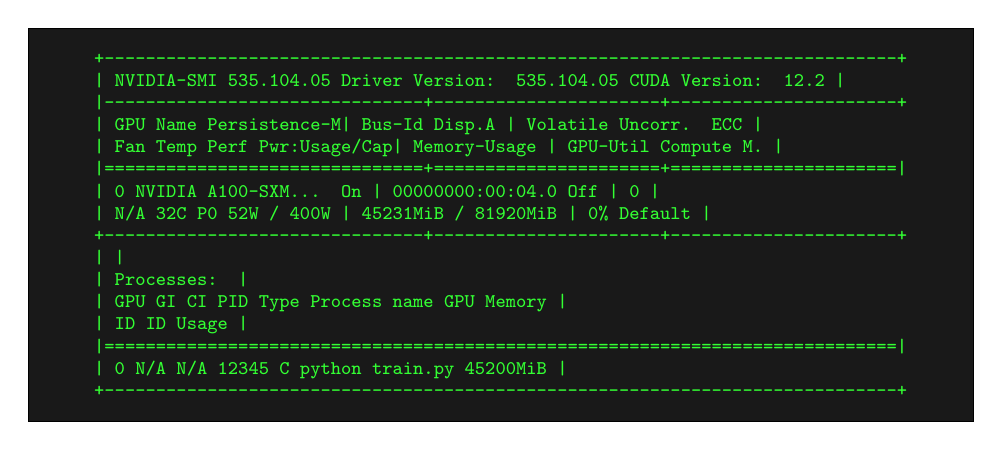
\begin{tikzpicture}[scale=0.9]
    % nvidia-smi 输出示意
    \node[draw, rectangle, fill=black!90, text=green!80, font=\ttfamily\scriptsize, 
          align=left, minimum width=12cm, minimum height=5cm] at (0, 0) {
+-----------------------------------------------------------------------------+\\
| NVIDIA-SMI 535.104.05   Driver Version: 535.104.05   CUDA Version: 12.2     |\\
|-------------------------------+----------------------+----------------------+\\
| GPU  Name        Persistence-M| Bus-Id        Disp.A | Volatile Uncorr. ECC |\\
| Fan  Temp  Perf  Pwr:Usage/Cap|         Memory-Usage | GPU-Util  Compute M. |\\
|===============================+======================+======================|\\
|   0  NVIDIA A100-SXM...  On   | 00000000:00:04.0 Off |                    0 |\\
| N/A   32C    P0    52W / 400W |  45231MiB / 81920MiB |      0\%      Default |\\
+-------------------------------+----------------------+----------------------+\\
|                                                                             |\\
| Processes:                                                                  |\\
|  GPU   GI   CI        PID   Type   Process name                  GPU Memory |\\
|        ID   ID                                                   Usage      |\\
|=============================================================================|\\
|    0   N/A  N/A     12345      C   python train.py                45200MiB |\\
+-----------------------------------------------------------------------------+
    };
\end{tikzpicture}
\caption{\texttt{nvidia-smi}输出示例：显示GPU型号、显存使用、运行中的进程}
\end{figure}

\paragraph{文件传输}\mbox{}\par\nopagebreak

\begin{lstlisting}[language=bash, caption=在本地和服务器之间传输文件]
# 从本地上传到服务器
scp local_file.py zhangsan@server:/home/zhangsan/project/

# 从服务器下载到本地
scp zhangsan@server:/home/zhangsan/results.csv ./

# 上传整个文件夹（-r 递归）
scp -r ./my_project zhangsan@server:/home/zhangsan/

# 如果配置了SSH config，可以用别名
scp local_file.py lab:/home/zhangsan/project/
\end{lstlisting}

% ------------------------------------------------------------------------------------
\section*{Git版本控制}
\addcontentsline{toc}{section}{Git版本控制}
% ------------------------------------------------------------------------------------

Git是代码版本管理的标准工具。即使只有你一个人写代码，也强烈建议用Git。

\paragraph{为什么要用Git？}

Git 记录你的每一次修改，所以任何时候都可以回退到之前的某个版本；有了这层保险，你就不必担心改坏代码——改坏了就退回去。它还解决了另一个很实际的问题：代码要在本地和服务器等多台机器之间来回同步，多人合作时还要合并各自的改动，靠手工拷贝文件很快就会乱套，而 Git 正是为此设计的。

\paragraph{Git基本工作流程}\mbox{}\par\nopagebreak

\begin{figure}[H]
\centering
\begin{tikzpicture}[>=stealth, scale=0.85,
    box/.style={draw, rounded corners, minimum width=2.2cm, minimum height=1cm, align=center}]
    
    % 三个区域
    \node[box, fill=blue!20] (work) at (0, 0) {工作目录\\Working};
    \node[box, fill=green!20] (stage) at (5, 0) {暂存区\\Staging};
    \node[box, fill=orange!20] (repo) at (10, 0) {本地仓库\\Repository};
    \node[box, fill=purple!20] (remote) at (10, -3) {远程仓库\\GitHub/GitLab};
    
    % 箭头
    \draw[->, thick] (work) -- node[above, font=\small] {\texttt{git add}} (stage);
    \draw[->, thick] (stage) -- node[above, font=\small] {\texttt{git commit}} (repo);
    \draw[->, thick] (repo) -- node[right, font=\small] {\texttt{git push}} (remote);
    \draw[->, thick] (remote) -- node[left, font=\small] {\texttt{git pull}} ++(-5, 0) -- (work);
    
\end{tikzpicture}
\caption{Git工作流程}
\end{figure}

\paragraph{常用Git命令}\mbox{}\par\nopagebreak

\begin{lstlisting}[language=bash, caption=Git常用命令]
# === 初始化 ===
git init                    # 在当前目录创建Git仓库
git clone <url>             # 克隆远程仓库

# === 日常使用 ===
git status                  # 查看当前状态（哪些文件改了）
git add .                   # 把所有修改添加到暂存区
git add train.py            # 只添加特定文件
git commit -m "描述信息"     # 提交，写清楚这次改了什么

# === 与远程同步 ===
git pull                    # 从远程拉取最新代码
git push                    # 把本地提交推送到远程

# === 查看历史 ===
git log --oneline           # 查看提交历史（简洁版）
git diff                    # 查看未暂存的修改
git diff --staged           # 查看已暂存的修改

# === 分支（进阶） ===
git branch                  # 查看分支
git checkout -b new_feature # 创建并切换到新分支
git merge new_feature       # 合并分支
\end{lstlisting}

\paragraph{典型工作流程示例}\mbox{}\par\nopagebreak

\begin{lstlisting}[language=bash, caption=一次完整的Git工作流程]
# 1. 开始工作前，先拉取最新代码
git pull

# 2. 写代码、做实验...

# 3. 查看改了哪些文件
git status

# 4. 添加修改
git add .

# 5. 提交，写清楚改了什么
git commit -m "增加学习率warmup功能"

# 6. 推送到远程（比如GitHub）
git push

# 现在你的代码就安全地保存在远程了！
\end{lstlisting}

\paragraph{.gitignore文件}

有些文件不应该加入Git（比如数据集、模型权重、临时文件）：

\begin{lstlisting}[language=bash, caption=.gitignore示例]
# .gitignore 文件内容

# 数据和模型（太大了）
data/
checkpoints/
*.pt
*.bin

# Python临时文件
__pycache__/
*.pyc
.ipynb_checkpoints/

# 环境和配置
.env
wandb/
outputs/

# 系统文件
.DS_Store
*.log
\end{lstlisting}

% ------------------------------------------------------------------------------------
\section*{Python环境管理：Conda}
\addcontentsline{toc}{section}{Python环境管理：Conda}
% ------------------------------------------------------------------------------------

服务器上可能有多个用户、多个项目，每个项目需要的Python版本和库可能不同。\textbf{Conda}帮你管理独立的Python环境。

\paragraph{为什么要用虚拟环境？}

不同项目常常需要不同版本的 PyTorch 和其他库，如果都装进同一个 Python 里，版本迟早会互相冲突，还会把系统自带的 Python 弄乱。虚拟环境把每个项目的依赖隔离开：各装各的版本，互不干扰；哪个环境出了问题，直接删掉重建就行，不会波及别的项目。

\paragraph{Conda基本命令}\mbox{}\par\nopagebreak

\begin{lstlisting}[language=bash, caption=Conda环境管理]
# === 创建环境 ===
conda create -n myenv python=3.10   # 创建名为myenv的环境，Python 3.10
conda activate myenv                 # 激活环境
conda deactivate                     # 退出环境

# === 查看环境 ===
conda env list                       # 列出所有环境
conda list                           # 列出当前环境的所有包

# === 安装包 ===
conda install numpy pandas           # 用conda安装
pip install torch transformers       # 用pip安装（conda没有的包）

# === 删除环境 ===
conda remove -n myenv --all          # 删除整个环境

# === 导出/导入环境 ===
conda env export > environment.yml   # 导出环境配置
conda env create -f environment.yml  # 从配置文件创建环境
\end{lstlisting}

\paragraph{典型深度学习环境配置}\mbox{}\par\nopagebreak

\begin{lstlisting}[language=bash, caption=配置一个深度学习环境]
# 1. 创建新环境
conda create -n llm python=3.10
conda activate llm

# 2. 安装PyTorch（去官网查对应CUDA版本的命令）
# https://pytorch.org/get-started/locally/
pip install torch torchvision torchaudio --index-url https://download.pytorch.org/whl/cu118

# 3. 安装常用库
pip install transformers datasets accelerate
pip install wandb tensorboard
pip install jupyter ipython

# 4. 验证安装
python -c "import torch; print(torch.cuda.is_available())"
# 应该输出 True
\end{lstlisting}

% ------------------------------------------------------------------------------------
\section*{CUDA 与 PyTorch 版本的坑}
\addcontentsline{toc}{section}{CUDA 与 PyTorch 版本的坑}
% ------------------------------------------------------------------------------------

\sidenoteplain{这一节是很多新手踩的最大坑：不理解CUDA版本、PyTorch版本、驱动版本之间的关系，随意升级，结果把组里老代码全搞挂了。}

在公用服务器上，\textbf{版本管理}是一个非常重要但经常被忽视的问题。理解下面这些概念，能帮你避免“一改配置全组遭殃”的惨剧。

\paragraph{三个版本的区别}\mbox{}\par\nopagebreak

\begin{table}[H]
\centering
\small
\renewcommand{\arraystretch}{1.4}
\begin{tabularx}{\textwidth}{l|X|l|l}
\toprule
\textbf{名称} & \textbf{是什么} & \textbf{谁负责安装} & \textbf{能否随意改} \\
\midrule
\textbf{NVIDIA驱动} & GPU的底层驱动 & 系统管理员 & \textcolor{red}{绝对不能！} \\
\textbf{CUDA Toolkit} & GPU编程工具包 & 系统或用户 & 谨慎（见下文） \\
\textbf{PyTorch CUDA版本} & PyTorch编译时用的CUDA & pip安装时选择 & 可以，但要匹配 \\
\bottomrule
\end{tabularx}
\caption{三种“CUDA版本”的区别}
\end{table}

\begin{keyidea}[版本兼容的关键原则]
三者的关系是分层的。\textbf{驱动}在最底层，同一台机器上只有一个；它向下兼容，所以驱动版本必须 $\geq$ CUDA Toolkit 版本。\textbf{CUDA Toolkit} 在中间，同一台机器上可以装多个版本。\textbf{PyTorch 的 CUDA 版本}在最上层，它必须与系统的 CUDA Toolkit 匹配。
\end{keyidea}

\paragraph{如何查看版本}\mbox{}\par\nopagebreak

\begin{lstlisting}[language=bash, caption=查看各种CUDA相关版本]
# 1. 查看NVIDIA驱动版本（nvidia-smi右上角）
nvidia-smi
# 输出: Driver Version: 535.104.05   CUDA Version: 12.2
#                                     ^^^^^^^^^^^^
#                        注意：这是驱动支持的最高CUDA版本，不是系统安装的CUDA

# 2. 查看系统安装的CUDA Toolkit版本
nvcc --version
# 输出: Cuda compilation tools, release 11.8, V11.8.89

# 3. 查看PyTorch使用的CUDA版本
python -c "import torch; print(torch.version.cuda)"
# 输出: 11.8

# 4. 验证PyTorch能否使用GPU
python -c "import torch; print(torch.cuda.is_available())"
# 输出: True  (如果是False，说明版本不匹配！)
\end{lstlisting}

\begin{remark}
\texttt{nvidia-smi}显示的“CUDA Version”容易让人误解。那是\textbf{驱动支持的最高CUDA版本}，不是你实际安装的CUDA版本。实际版本要用\texttt{nvcc --version}查看。
\end{remark}

\paragraph{什么是 \texttt{cuda:0}？}

当你写 \texttt{.to("cuda:0")} 时，\texttt{cuda:0}表示\textbf{第0号GPU}。

\begin{lstlisting}[language=Python, caption=GPU设备管理]
import torch

# 查看有几张GPU
print(torch.cuda.device_count())  # 比如输出 4，表示有4张卡

# 查看当前默认设备
print(torch.cuda.current_device())  # 通常是 0

# 把张量放到指定GPU
x = torch.randn(1000, 1000)
x = x.to("cuda:0")   # 放到第0张卡
x = x.to("cuda:1")   # 放到第1张卡
x = x.cuda()         # 等价于 .to("cuda:0")

# 指定默认GPU
torch.cuda.set_device(1)  # 之后.cuda()默认用第1张卡
\end{lstlisting}

\paragraph{使用 \texttt{CUDA\_VISIBLE\_DEVICES} 控制可见GPU}

在公用服务器上，你通常不能独占所有GPU。用环境变量控制你的程序能看到哪些卡：

\begin{lstlisting}[language=bash, caption=控制可见GPU]
# 只用第2张卡（编号从0开始）
CUDA_VISIBLE_DEVICES=2 python train.py

# 用第0和第3张卡
CUDA_VISIBLE_DEVICES=0,3 python train.py

# 此时在Python里：
# - torch.cuda.device_count() 返回 2
# - "cuda:0" 对应物理上的第0张卡
# - "cuda:1" 对应物理上的第3张卡

# 完全不用GPU（强制CPU）
CUDA_VISIBLE_DEVICES="" python train.py
\end{lstlisting}

\begin{warning}
\textbf{公用服务器的生存法则}：
\begin{enumerate}
    \item \textbf{永远不要升级系统的CUDA或驱动}——这会影响所有用户！
    \item \textbf{用Conda管理自己的PyTorch版本}——每个环境独立，不影响别人
    \item \textbf{用 \texttt{CUDA\_VISIBLE\_DEVICES} 指定GPU}——避免抢占别人正在用的卡
    \item \textbf{跑之前先 \texttt{nvidia-smi} 看一眼}——确认哪些卡空闲
\end{enumerate}
\end{warning}

\paragraph{版本不匹配的常见报错}\mbox{}\par\nopagebreak

\begin{table}[H]
\centering
\small
\renewcommand{\arraystretch}{1.4}
\begin{tabularx}{\textwidth}{X|X}
\toprule
\textbf{报错信息} & \textbf{可能原因} \\
\midrule
\texttt{CUDA error: no kernel image is available} & PyTorch的CUDA版本与GPU架构不匹配 \\
\texttt{torch.cuda.is\_available() = False} & PyTorch没装CUDA版本，或CUDA版本不匹配 \\
\texttt{CUDA out of memory} & 显存不够，或别人在用这张卡 \\
\texttt{RuntimeError: CUDA unknown error} & 驱动问题，尝试重启或联系管理员 \\
\bottomrule
\end{tabularx}
\caption{常见CUDA报错与原因}
\end{table}

\paragraph{安装正确版本的PyTorch}

安装命令要和系统的 CUDA 版本匹配。PyTorch 官网的安装页面会根据你选择的系统与 CUDA 版本生成对应的命令：
\begin{center}
\small\url{https://pytorch.org/get-started/locally/}
\end{center}

\begin{lstlisting}[language=bash, caption=根据CUDA版本安装PyTorch]
# 如果系统CUDA是11.8
pip install torch torchvision torchaudio --index-url https://download.pytorch.org/whl/cu118

# 如果系统CUDA是12.1
pip install torch torchvision torchaudio --index-url https://download.pytorch.org/whl/cu121

# CPU版本（没有GPU或想强制用CPU）
pip install torch torchvision torchaudio --index-url https://download.pytorch.org/whl/cpu
\end{lstlisting}

\begin{example}[一个典型的“版本地狱”场景]
师兄的代码在服务器上跑得好好的。你为了跑一个新论文的代码，把系统 CUDA 从 11.8 升级到 12.2。结果，师兄的 PyTorch 是 cu118 版本，现在 \texttt{torch.cuda.is\_available()} 返回 False；师姐用的 TensorFlow 也挂了；导师开始问为什么大家的实验都跑不了了……

正确的做法是不碰系统 CUDA：用 Conda 创建一个新环境，在里面装 cu118 版本的 PyTorch（驱动向下兼容，没有问题）；如果新代码确实需要更新的 CUDA，就联系管理员，在不影响现有环境的前提下另外添加一个版本。
\end{example}

% ------------------------------------------------------------------------------------
\section*{后台运行：Screen和Tmux}
\addcontentsline{toc}{section}{后台运行：Screen和Tmux}
% ------------------------------------------------------------------------------------

SSH断开后，正在运行的程序会被终止。用\texttt{screen}或\texttt{tmux}可以让程序在后台持续运行。

\paragraph{Screen基本用法}\mbox{}\par\nopagebreak

\begin{lstlisting}[language=bash, caption=Screen使用方法]
# 创建新的screen会话
screen -S train          # 创建名为train的会话

# 在screen里运行训练
python train.py

# 断开screen（程序继续运行）
# 按 Ctrl+A，然后按 D

# 重新连接
screen -r train          # 连接到train会话

# 查看所有会话
screen -ls

# 结束会话
exit                     # 在screen里输入exit
# 或者 screen -X -S train quit
\end{lstlisting}

\paragraph{Tmux基本用法}

Tmux功能更强大，推荐使用：

\begin{lstlisting}[language=bash, caption=Tmux使用方法]
# 创建新会话
tmux new -s train

# 断开（detach）
# 按 Ctrl+B，然后按 D

# 重新连接
tmux attach -t train
# 或简写
tmux a -t train

# 查看所有会话
tmux ls

# 结束会话
tmux kill-session -t train
\end{lstlisting}

\begin{figure}[htbp]
\centering
\begin{tikzpicture}[>=stealth, scale=0.85]

    % 服务器框
    \node[draw, rectangle, fill=blue!10,
          minimum width=10cm, minimum height=4cm] (server) at (0, 0) {};
    \node[above] at (0, 2.2) {服务器};

    % Tmux 会话
\node[
    draw,
    rectangle,
    fill=green!20,
    minimum width=4cm,
    minimum height=1.5cm,
    align=center
] (tmux1) at (-2, 0.5)
    {\texttt{tmux: train}\\\texttt{python train.py}};

\node[
    draw,
    rectangle,
    fill=orange!20,
    minimum width=4cm,
    minimum height=1.5cm,
    align=center
] (tmux2) at (-2, -1.5)
    {\texttt{tmux: eval}\\\texttt{python eval.py}};


    % 用户
    \node[draw, circle, fill=yellow!30] (user) at (6, 0) {你};

    % SSH 连线
    \draw[<->, thick] (user) -- node[above] {SSH} (2, 0);

    % 注释
    \node[font=\small, gray, align=center] at (6, -1.6) {SSH断开后\\tmux里的程序\\继续运行};

\end{tikzpicture}
\caption{Tmux让程序在后台持续运行}
\end{figure}


% ------------------------------------------------------------------------------------
\section*{集群任务调度：SLURM}
\addcontentsline{toc}{section}{集群任务调度：SLURM}
% ------------------------------------------------------------------------------------

如果你使用学校的计算集群（HPC），通常需要通过\textbf{SLURM}提交任务。SLURM会把你的任务排队，等有空闲GPU时自动运行。

\paragraph{SLURM基本概念}

先认识四个词。集群由许多台物理服务器组成，每一台叫一个\textbf{节点}（Node）；管理员把节点分成若干组，比如 gpu 分区、cpu 分区，每一组叫一个\textbf{分区}（Partition）。你提交给集群的任务叫\textbf{作业}（Job），而描述这个作业需要什么资源、要运行什么命令的文件，就是作业\textbf{脚本}（Script）。

\paragraph{查看集群状态}\mbox{}\par\nopagebreak

\begin{lstlisting}[language=bash, caption=SLURM常用查询命令]
# 查看所有分区和节点状态
sinfo

# 查看队列中的作业
squeue

# 只看自己的作业
squeue -u $USER

# 查看作业详细信息
scontrol show job <job_id>

# 查看历史作业
sacct -u $USER --starttime=2024-01-01
\end{lstlisting}

\paragraph{编写SLURM脚本}\mbox{}\par\nopagebreak

\begin{lstlisting}[language=bash, caption=SLURM作业脚本示例（train.slurm）]
#!/bin/bash
#SBATCH --job-name=llm_train        # 作业名称
#SBATCH --partition=gpu             # 分区（队列）名称
#SBATCH --nodes=1                   # 节点数
#SBATCH --ntasks-per-node=1         # 每节点任务数
#SBATCH --cpus-per-task=8           # 每任务CPU核数
#SBATCH --gres=gpu:4                # GPU数量
#SBATCH --mem=64G                   # 内存
#SBATCH --time=24:00:00             # 最大运行时间
#SBATCH --output=logs/%j.out        # 标准输出文件（%j是作业ID）
#SBATCH --error=logs/%j.err         # 错误输出文件

# 加载环境
source ~/.bashrc
conda activate llm

# 进入工作目录
cd /home/zhangsan/project

# 运行训练
python train.py \
    --model_name llama-7b \
    --batch_size 4 \
    --learning_rate 2e-5 \
    --num_epochs 3
\end{lstlisting}

\paragraph{提交和管理作业}\mbox{}\par\nopagebreak

\begin{lstlisting}[language=bash, caption=提交和管理SLURM作业]
# 提交作业
sbatch train.slurm
# 返回：Submitted batch job 12345

# 查看作业状态
squeue -u $USER
# JOBID  PARTITION  NAME       USER      ST  TIME  NODES  NODELIST
# 12345  gpu        llm_train  zhangsan  R   1:23  1      gpu-node-01

# 取消作业
scancel 12345

# 取消自己的所有作业
scancel -u $USER
\end{lstlisting}

\paragraph{交互式调试}

有时候需要交互式地调试代码，可以申请一个交互式会话：

\begin{lstlisting}[language=bash, caption=申请交互式GPU会话]
# 申请1张GPU，2小时
srun --partition=gpu --gres=gpu:1 --time=2:00:00 --pty bash

# 现在你在一个有GPU的节点上了
nvidia-smi          # 可以看到GPU
python train.py     # 可以直接运行代码

# 退出交互式会话
exit
\end{lstlisting}

\paragraph{多GPU训练脚本示例}\mbox{}\par\nopagebreak

\begin{lstlisting}[language=bash, caption=多GPU分布式训练脚本]
#!/bin/bash
#SBATCH --job-name=llm_ddp
#SBATCH --partition=gpu
#SBATCH --nodes=2                   # 2个节点
#SBATCH --ntasks-per-node=4         # 每节点4个任务（对应4张GPU）
#SBATCH --gres=gpu:4                # 每节点4张GPU
#SBATCH --cpus-per-task=4
#SBATCH --mem=128G
#SBATCH --time=48:00:00
#SBATCH --output=logs/%j.out

source ~/.bashrc
conda activate llm

# 设置分布式训练环境变量
export MASTER_ADDR=$(scontrol show hostnames $SLURM_JOB_NODELIST | head -n 1)
export MASTER_PORT=29500
export WORLD_SIZE=$SLURM_NTASKS

# 使用torchrun启动分布式训练
srun torchrun \
    --nnodes=$SLURM_NNODES \
    --nproc_per_node=4 \
    --rdzv_id=$SLURM_JOB_ID \
    --rdzv_backend=c10d \
    --rdzv_endpoint=$MASTER_ADDR:$MASTER_PORT \
    train.py \
    --batch_size 8 \
    --gradient_accumulation_steps 4
\end{lstlisting}

% ------------------------------------------------------------------------------------
\section*{实用技巧汇总}
\addcontentsline{toc}{section}{实用技巧汇总}
% ------------------------------------------------------------------------------------

\paragraph{训练监控}\mbox{}\par\nopagebreak

\begin{lstlisting}[language=bash, caption=监控训练过程]
# 实时查看训练日志
tail -f logs/12345.out

# 实时监控GPU
watch -n 1 nvidia-smi

# 使用wandb或tensorboard可视化
# 在训练代码中集成wandb
tensorboard --logdir=./runs --port=6006

# 如果在服务器上运行tensorboard，需要端口转发
# 在本地运行：
ssh -L 6006:localhost:6006 lab
# 然后在本地浏览器打开 http://localhost:6006
\end{lstlisting}

\paragraph{常见问题排查}\mbox{}\par\nopagebreak

\begin{table}[H]
\centering
\small
\renewcommand{\arraystretch}{1.4}
\begin{tabular}{l|l}
\toprule
\textbf{问题} & \textbf{解决方法} \\
\midrule
CUDA out of memory & 减小batch size，用梯度累积 \\
SSH连接断开程序终止 & 用tmux或screen \\
找不到GPU & 检查\texttt{CUDA\_VISIBLE\_DEVICES}环境变量 \\
权限不够 & 检查文件权限，用\texttt{chmod} \\
磁盘空间不足 & \texttt{du -sh *}找大文件，清理checkpoint \\
作业一直排队 & \texttt{sinfo}看资源，考虑换分区或减少资源请求 \\
\bottomrule
\end{tabular}
\caption{常见问题与解决方法}
\end{table}

\paragraph{一个完整的实验流程}\mbox{}\par\nopagebreak

\begin{lstlisting}[language=bash, caption=从零开始的完整实验流程]
# === 1. 连接服务器 ===
ssh lab

# === 2. 创建项目目录 ===
mkdir -p ~/projects/my_llm_exp
cd ~/projects/my_llm_exp

# === 3. 克隆代码 ===
git clone https://github.com/yourname/llm-finetune.git
cd llm-finetune

# === 4. 创建环境 ===
conda create -n myexp python=3.10
conda activate myexp
pip install -r requirements.txt

# === 5. 准备数据 ===
mkdir -p data
# 上传或下载数据到 data/ 目录

# === 6. 测试代码（交互式，小数据） ===
srun --partition=gpu --gres=gpu:1 --time=1:00:00 --pty bash
python train.py --debug --max_samples 100
exit

# === 7. 提交正式训练 ===
mkdir -p logs
sbatch train.slurm

# === 8. 监控训练 ===
squeue -u $USER
tail -f logs/<job_id>.out

# === 9. 训练完成后，下载结果 ===
# 在本地：
scp -r lab:~/projects/my_llm_exp/checkpoints ./
\end{lstlisting}

% ------------------------------------------------------------------------------------
\section*{推荐的目录结构}
\addcontentsline{toc}{section}{推荐的目录结构}
% ------------------------------------------------------------------------------------

一个组织良好的项目目录让你的实验更容易管理：

\begin{lstlisting}[language=bash, caption=推荐的项目目录结构]
my_project/
|-- data/                    # 数据（通常不加入git）
|   |-- train.json
|   |-- eval.json
|
|-- src/                     # 源代码
|   |-- model.py
|   |-- train.py
|   |-- eval.py
|   |-- utils.py
|
|-- configs/                 # 配置文件
|   |-- train_7b.yaml
|   |-- train_13b.yaml
|
|-- scripts/                 # 运行脚本
|   |-- train.slurm
|   |-- eval.slurm
|
|-- checkpoints/             # 模型权重（不加入git）
|-- logs/                    # 日志（不加入git）
|-- outputs/                 # 输出结果
|
|-- requirements.txt         # Python依赖
|-- README.md               # 项目说明
|-- .gitignore              # Git忽略文件
\end{lstlisting}

\begin{remark}
再养成几个习惯：代码改动及时 commit；重要的实验把配置和结果一起记下来；checkpoint 很占空间，要定期清理；给文件和变量起有意义的名字。这些习惯会在你做毕设或发论文时帮大忙。
\end{remark}

% ------------------------------------------------------------------------------------
\section*{常用工具库速览}
\addcontentsline{toc}{section}{常用工具库速览}
% ------------------------------------------------------------------------------------

深度学习生态有大量优秀的开源工具。这里介绍最常用的几类，帮你快速上手。

\subsection*{Hugging Face 生态}

\sidenoteplain{\textbf{Hugging Face}：由法国人Clément Delangue等于2016年创立，最初是一个聊天机器人。2019年开源Transformers库后爆发式增长，如今已成为AI开源社区的``GitHub''，托管超过50万个模型。公司估值超40亿美元。}

Hugging Face是目前最流行的NLP/LLM工具生态，几乎是必学的。

\paragraph{Transformers：模型加载与推理}\mbox{}\par\nopagebreak

\begin{lstlisting}[language=Python, caption=使用Transformers加载和使用模型]
from transformers import AutoTokenizer, AutoModelForCausalLM
import torch

# 加载模型和分词器（会自动从Hugging Face下载）
model_name = "meta-llama/Llama-2-7b-hf"  # 或本地路径
tokenizer = AutoTokenizer.from_pretrained(model_name)
model = AutoModelForCausalLM.from_pretrained(
    model_name,
    torch_dtype=torch.float16,  # 半精度节省显存
    device_map="auto"           # 自动分配到GPU
)

# 生成文本
prompt = "人工智能的未来发展方向是"
inputs = tokenizer(prompt, return_tensors="pt").to(model.device)
outputs = model.generate(
    **inputs,
    max_new_tokens=100,
    temperature=0.7,
    do_sample=True
)
print(tokenizer.decode(outputs[0], skip_special_tokens=True))
\end{lstlisting}

\paragraph{PEFT：参数高效微调（LoRA等）}

PEFT（Parameter-Efficient Fine-Tuning）库让你用几行代码就能实现LoRA微调：

\begin{lstlisting}[language=Python, caption=使用PEFT进行LoRA微调]
from transformers import AutoModelForCausalLM, AutoTokenizer, TrainingArguments
from peft import LoraConfig, get_peft_model, TaskType
from trl import SFTTrainer

# 1. 加载基础模型
model = AutoModelForCausalLM.from_pretrained(
    "meta-llama/Llama-2-7b-hf",
    torch_dtype=torch.float16,
    device_map="auto"
)

# 2. 配置LoRA
lora_config = LoraConfig(
    task_type=TaskType.CAUSAL_LM,
    r=8,                        # LoRA秩
    lora_alpha=16,              # 缩放因子
    lora_dropout=0.05,
    target_modules=["q_proj", "v_proj"],  # 对哪些层应用LoRA
)

# 3. 创建PEFT模型
model = get_peft_model(model, lora_config)
model.print_trainable_parameters()
# 输出类似：trainable params: 4,194,304 || all params: 6,742,609,920 || trainable%: 0.0622

# 4. 训练（使用trl的SFTTrainer更方便）
trainer = SFTTrainer(
    model=model,
    train_dataset=dataset,
    args=TrainingArguments(
        output_dir="./output",
        per_device_train_batch_size=4,
        gradient_accumulation_steps=4,
        num_train_epochs=3,
        learning_rate=2e-4,
        fp16=True,
        logging_steps=10,
        save_steps=100,
    ),
)
trainer.train()

# 5. 保存LoRA权重（只保存增量，很小）
model.save_pretrained("./lora_weights")
\end{lstlisting}

\paragraph{Datasets：数据加载与处理}\mbox{}\par\nopagebreak

\begin{lstlisting}[language=Python, caption=使用Datasets处理数据]
from datasets import load_dataset, Dataset

# 加载公开数据集
dataset = load_dataset("tatsu-lab/alpaca")  # 指令微调数据

# 加载本地JSON文件
dataset = load_dataset("json", data_files="data/train.json")

# 从Python字典创建
data = {
    "instruction": ["写一首诗", "翻译成英文"],
    "input": ["关于春天", "你好世界"],
    "output": ["春风拂面...", "Hello World"]
}
dataset = Dataset.from_dict(data)

# 数据预处理
def preprocess(example):
    prompt = f"### 指令:\n{example['instruction']}\n### 回答:\n"
    return {"text": prompt + example["output"]}

dataset = dataset.map(preprocess)

# 划分训练集和验证集
dataset = dataset.train_test_split(test_size=0.1)
\end{lstlisting}

\begin{table}[htbp]
\centering
\small
\renewcommand{\arraystretch}{1.3}
\begin{tabular}{l|l|l}
\toprule
\textbf{库} & \textbf{功能} & \textbf{安装} \\
\midrule
transformers & 模型加载、推理、训练 & \texttt{pip install transformers} \\
peft & LoRA、QLoRA等高效微调 & \texttt{pip install peft} \\
datasets & 数据集加载与处理 & \texttt{pip install datasets} \\
accelerate & 分布式训练、混合精度 & \texttt{pip install accelerate} \\
trl & RLHF、SFT训练器 & \texttt{pip install trl} \\
bitsandbytes & 4/8-bit量化 & \texttt{pip install bitsandbytes} \\
\bottomrule
\end{tabular}
\caption{Hugging Face生态常用库}
\end{table}

\subsection*{量化推理：让大模型在小显卡上跑}

显存不够时，量化是最直接的解决方案。

\paragraph{BitsAndBytes：4-bit/8-bit量化}\mbox{}\par\nopagebreak

\begin{lstlisting}[language=Python, caption=4-bit量化加载模型]
from transformers import AutoModelForCausalLM, AutoTokenizer, BitsAndBytesConfig

# 配置4-bit量化
bnb_config = BitsAndBytesConfig(
    load_in_4bit=True,                    # 4-bit加载
    bnb_4bit_quant_type="nf4",           # NormalFloat4量化
    bnb_4bit_compute_dtype=torch.float16, # 计算时用FP16
    bnb_4bit_use_double_quant=True,      # 二次量化，进一步压缩
)

# 加载量化模型
model = AutoModelForCausalLM.from_pretrained(
    "meta-llama/Llama-2-7b-hf",
    quantization_config=bnb_config,
    device_map="auto"
)
# 原本需要14GB显存，现在只需要约4GB！
\end{lstlisting}

\paragraph{QLoRA：量化 + LoRA}

QLoRA结合了量化和LoRA，可以在单张消费级显卡上微调大模型：

\begin{lstlisting}[language=Python, caption=QLoRA微调]
from peft import prepare_model_for_kbit_training

# 1. 加载4-bit量化模型
model = AutoModelForCausalLM.from_pretrained(
    "meta-llama/Llama-2-7b-hf",
    quantization_config=bnb_config,
    device_map="auto"
)

# 2. 准备模型进行k-bit训练
model = prepare_model_for_kbit_training(model)

# 3. 添加LoRA
model = get_peft_model(model, lora_config)

# 现在可以在RTX 3080 (10GB) 上微调7B模型了！
\end{lstlisting}

\paragraph{GPTQ/AWQ：更高效的量化}\mbox{}\par\nopagebreak

\begin{lstlisting}[language=Python, caption=加载GPTQ量化模型]
from transformers import AutoModelForCausalLM

# GPTQ量化模型（需要预先量化好的权重）
model = AutoModelForCausalLM.from_pretrained(
    "TheBloke/Llama-2-7B-GPTQ",  # 社区量化的模型
    device_map="auto"
)
\end{lstlisting}

\begin{table}[htbp]
\centering
\small
\renewcommand{\arraystretch}{1.3}
\begin{tabular}{l|c|c|l}
\toprule
\textbf{量化方法} & \textbf{精度} & \textbf{7B模型显存} & \textbf{特点} \\
\midrule
无量化 (FP16) & 高 & 14 GB & 基准 \\
BitsAndBytes 8-bit & 较高 & 8 GB & 简单易用 \\
BitsAndBytes 4-bit & 中等 & 4-5 GB & 配合LoRA微调 \\
GPTQ 4-bit & 中等 & 4 GB & 推理快，需预量化 \\
AWQ 4-bit & 中等 & 4 GB & 推理更快 \\
\bottomrule
\end{tabular}
\caption{常见量化方法对比}
\end{table}

\subsection*{高效推理框架}

当你需要部署模型提供服务时，这些框架能大幅提升吞吐量。

\paragraph{vLLM：高吞吐量推理}

vLLM使用PagedAttention技术，显著提升推理效率：

\begin{lstlisting}[language=Python, caption=使用vLLM进行高效推理]
from vllm import LLM, SamplingParams

# 加载模型
llm = LLM(
    model="meta-llama/Llama-2-7b-hf",
    tensor_parallel_size=1,  # GPU数量
    dtype="float16"
)

# 配置采样参数
sampling_params = SamplingParams(
    temperature=0.7,
    top_p=0.9,
    max_tokens=256
)

# 批量推理（vLLM会自动优化批处理）
prompts = [
    "北京是中国的",
    "机器学习的核心思想是",
    "今天天气很好，我想"
]
outputs = llm.generate(prompts, sampling_params)

for output in outputs:
    print(output.outputs[0].text)
\end{lstlisting}

\paragraph{启动vLLM API服务}\mbox{}\par\nopagebreak

\begin{lstlisting}[language=bash, caption=启动vLLM服务器]
# 启动OpenAI兼容的API服务
python -m vllm.entrypoints.openai.api_server \
    --model meta-llama/Llama-2-7b-hf \
    --port 8000

# 然后可以用OpenAI的客户端调用
# curl http://localhost:8000/v1/completions ...
\end{lstlisting}

\paragraph{其他推理框架}\mbox{}\par\nopagebreak

\begin{table}[H]
\centering
\small
\renewcommand{\arraystretch}{1.3}
\begin{tabular}{l|l|l}
\toprule
\textbf{框架} & \textbf{特点} & \textbf{适用场景} \\
\midrule
vLLM & PagedAttention，高吞吐 & 生产部署 \\
Text Generation Inference & Hugging Face官方 & 容器化部署 \\
llama.cpp & CPU/低端GPU推理 & 本地运行、边缘设备 \\
Ollama & 一键运行本地模型 & 个人使用、快速体验 \\
\bottomrule
\end{tabular}
\caption{常见推理框架对比}
\end{table}

\subsection*{LangChain：构建LLM应用}

LangChain是构建LLM应用的流行框架，提供了链式调用、RAG、Agent等功能。

\paragraph{基本使用}\mbox{}\par\nopagebreak

\begin{lstlisting}[language=Python, caption=LangChain基本使用]
from langchain_openai import ChatOpenAI
from langchain_core.prompts import ChatPromptTemplate
from langchain_core.output_parsers import StrOutputParser

# 1. 创建模型（可以用OpenAI或本地模型）
llm = ChatOpenAI(
    model="gpt-3.5-turbo",
    temperature=0.7
)

# 2. 创建提示模板
prompt = ChatPromptTemplate.from_messages([
    ("system", "你是一个专业的{role}。"),
    ("user", "{question}")
])

# 3. 创建链（Chain）
chain = prompt | llm | StrOutputParser()

# 4. 运行
response = chain.invoke({
    "role": "Python程序员",
    "question": "如何读取CSV文件？"
})
print(response)
\end{lstlisting}

\paragraph{RAG：检索增强生成}

RAG让模型能够基于你的文档回答问题：

\begin{lstlisting}[language=Python, caption=使用LangChain构建RAG系统]
from langchain_community.document_loaders import PyPDFLoader
from langchain.text_splitter import RecursiveCharacterTextSplitter
from langchain_community.vectorstores import FAISS
from langchain_openai import OpenAIEmbeddings
from langchain.chains import RetrievalQA

# 1. 加载文档
loader = PyPDFLoader("paper.pdf")
documents = loader.load()

# 2. 切分文档
text_splitter = RecursiveCharacterTextSplitter(
    chunk_size=1000,
    chunk_overlap=200
)
splits = text_splitter.split_documents(documents)

# 3. 创建向量存储
embeddings = OpenAIEmbeddings()
vectorstore = FAISS.from_documents(splits, embeddings)

# 4. 创建检索QA链
qa_chain = RetrievalQA.from_chain_type(
    llm=ChatOpenAI(model="gpt-3.5-turbo"),
    chain_type="stuff",
    retriever=vectorstore.as_retriever(search_kwargs={"k": 3})
)

# 5. 提问
answer = qa_chain.invoke("这篇论文的主要贡献是什么？")
print(answer)
\end{lstlisting}

\begin{figure}[htbp]
\centering
\begin{tikzpicture}[>=stealth, scale=0.8,
    box/.style={draw, rounded corners, minimum width=2cm, minimum height=1cm, align=center, font=\small}]
    
    % RAG流程
    \node[box, fill=blue!20] (query) at (0, 0) {用户问题};
    \node[box, fill=green!20] (embed) at (3, 0) {向量化};
    \node[box, fill=orange!20] (search) at (6, 0) {检索相关\\文档};
    \node[box, fill=purple!20] (llm) at (9, 0) {LLM生成\\回答};
    \node[box, fill=red!20] (answer) at (12, 0) {最终答案};
    
    % 向量数据库
    \node[box, fill=yellow!20] (db) at (6, -2.5) {向量数据库\\(文档切片)};
    
    % 箭头
    \draw[->, thick] (query) -- (embed);
    \draw[->, thick] (embed) -- (search);
    \draw[->, thick] (search) -- (llm);
    \draw[->, thick] (llm) -- (answer);
    \draw[->, thick] (search) -- (db);
    \draw[->, thick] (db) -- (search);
    
\end{tikzpicture}
\caption{RAG（检索增强生成）流程}
\end{figure}

\paragraph{Agent：让LLM使用工具}

Agent 可以让 LLM 调用外部工具（搜索、计算器、代码执行等）。下面用到的 ReAct 提示模板，实现的正是第 12 章里姚顺雨 2022 年提出的那套节奏：让模型交替地``想一步''和``做一步''，把工具返回的观察再喂回推理：

\begin{lstlisting}[language=Python, caption=创建简单的Agent]
from langchain_openai import ChatOpenAI
from langchain.agents import tool, AgentExecutor, create_react_agent
from langchain import hub

# 1. 定义工具
@tool
def search_weather(city: str) -> str:
    """查询城市天气"""
    # 实际应该调用天气API
    return f"{city}今天晴，气温25度"

@tool  
def calculate(expression: str) -> str:
    """计算数学表达式"""
    return str(eval(expression))

tools = [search_weather, calculate]

# 2. 创建Agent
llm = ChatOpenAI(model="gpt-4", temperature=0)
prompt = hub.pull("hwchase17/react")  # 使用ReAct提示模板
agent = create_react_agent(llm, tools, prompt)

# 3. 创建执行器
agent_executor = AgentExecutor(
    agent=agent, 
    tools=tools, 
    verbose=True  # 打印推理过程
)

# 4. 运行
response = agent_executor.invoke({
    "input": "北京今天天气怎么样？如果温度乘以2是多少？"
})
print(response["output"])
\end{lstlisting}

\subsection*{实验追踪：Weights \& Biases}

W\&B（wandb）帮你记录实验、可视化训练曲线、比较不同配置：

\begin{lstlisting}[language=Python, caption=使用W\&B追踪实验]
import wandb

# 1. 初始化（第一次需要登录：wandb login）
wandb.init(
    project="llm-finetune",      # 项目名
    name="lora-r8-lr2e4",        # 本次实验名
    config={                      # 记录超参数
        "model": "llama-7b",
        "lora_r": 8,
        "learning_rate": 2e-4,
        "batch_size": 4,
    }
)

# 2. 在训练循环中记录指标
for epoch in range(num_epochs):
    for batch in dataloader:
        loss = train_step(batch)
        wandb.log({
            "train/loss": loss,
            "train/epoch": epoch
        })
    
    # 验证
    val_loss = evaluate()
    wandb.log({"val/loss": val_loss})

# 3. 结束
wandb.finish()

# 如果使用HuggingFace Trainer，直接设置report_to="wandb"即可
\end{lstlisting}

\begin{figure}[htbp]
\centering
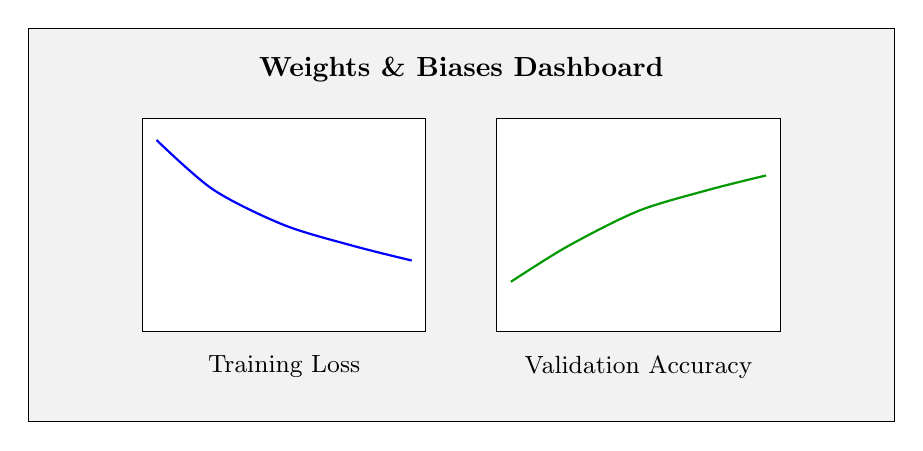
\begin{tikzpicture}[scale=0.9]
    % W&B界面示意
    \node[draw, rectangle, fill=gray!10, minimum width=11cm, minimum height=5cm] at (0, 0) {};
    
    % 图表区域
    \draw[fill=white] (-4.5, -1.5) rectangle (-0.5, 1.5);
    \draw[thick, blue, smooth] plot coordinates {(-4.3, 1.2) (-3.5, 0.5) (-2.5, 0) (-1.5, -0.3) (-0.7, -0.5)};
    \node[font=\small] at (-2.5, -2) {Training Loss};
    
    \draw[fill=white] (0.5, -1.5) rectangle (4.5, 1.5);
    \draw[thick, green!60!black, smooth] plot coordinates {(0.7, -0.8) (1.5, -0.3) (2.5, 0.2) (3.5, 0.5) (4.3, 0.7)};
    \node[font=\small] at (2.5, -2) {Validation Accuracy};
    
    % 标题
    \node[font=\bfseries] at (0, 2.2) {Weights \& Biases Dashboard};
    
\end{tikzpicture}
\caption{W\&B自动生成训练曲线和实验对比}
\end{figure}

\subsection*{工具库速查表}

\begin{table}[htbp]
\centering
\small
\renewcommand{\arraystretch}{1.4}
\begin{tabular}{l|l|l}
\toprule
\textbf{任务} & \textbf{推荐工具} & \textbf{一句话说明} \\
\midrule
\multicolumn{3}{c}{\textit{模型训练与微调}} \\
\midrule
加载预训练模型 & Transformers & \texttt{AutoModel.from\_pretrained()} \\
LoRA/QLoRA微调 & PEFT + BitsAndBytes & 低显存微调大模型 \\
分布式训练 & Accelerate / DeepSpeed & 多卡/多机训练 \\
RLHF训练 & TRL & PPO、DPO实现 \\
\midrule
\multicolumn{3}{c}{\textit{推理与部署}} \\
\midrule
高效批量推理 & vLLM & PagedAttention，高吞吐 \\
本地快速体验 & Ollama & \texttt{ollama run llama2} \\
CPU/边缘推理 & llama.cpp & C++实现，无需GPU \\
\midrule
\multicolumn{3}{c}{\textit{应用开发}} \\
\midrule
构建LLM应用 & LangChain & 链式调用、RAG、Agent \\
向量数据库 & FAISS / Chroma & 存储和检索文档向量 \\
\midrule
\multicolumn{3}{c}{\textit{实验管理}} \\
\midrule
实验追踪 & Weights \& Biases & 记录指标、可视化 \\
可视化 & TensorBoard & \texttt{tensorboard --logdir=runs} \\
\bottomrule
\end{tabular}
\caption{常用工具库速查}
\end{table}

\subsection*{一个完整的微调示例}

把前面的工具组合起来，这是一个完整的LoRA微调脚本：

\begin{lstlisting}[language=Python, caption=完整的LoRA微调脚本]
"""
LLaMA LoRA微调完整示例
运行: python finetune.py
"""
import torch
from datasets import load_dataset
from transformers import (
    AutoModelForCausalLM,
    AutoTokenizer,
    TrainingArguments,
    BitsAndBytesConfig,
)
from peft import LoraConfig, get_peft_model, prepare_model_for_kbit_training
from trl import SFTTrainer
import wandb

# ============ 配置 ============
MODEL_NAME = "meta-llama/Llama-2-7b-hf"
OUTPUT_DIR = "./output"
LORA_R = 8
LORA_ALPHA = 16
LEARNING_RATE = 2e-4
BATCH_SIZE = 4
GRAD_ACCUM = 4
NUM_EPOCHS = 3
MAX_SEQ_LEN = 1024

# ============ 初始化W&B ============
wandb.init(project="llm-finetune", name="lora-alpaca")

# ============ 加载模型（4-bit量化）============
bnb_config = BitsAndBytesConfig(
    load_in_4bit=True,
    bnb_4bit_quant_type="nf4",
    bnb_4bit_compute_dtype=torch.float16,
)

model = AutoModelForCausalLM.from_pretrained(
    MODEL_NAME,
    quantization_config=bnb_config,
    device_map="auto",
)
tokenizer = AutoTokenizer.from_pretrained(MODEL_NAME)
tokenizer.pad_token = tokenizer.eos_token

# ============ 配置LoRA ============
model = prepare_model_for_kbit_training(model)
lora_config = LoraConfig(
    r=LORA_R,
    lora_alpha=LORA_ALPHA,
    lora_dropout=0.05,
    target_modules=["q_proj", "v_proj", "k_proj", "o_proj"],
    task_type="CAUSAL_LM",
)
model = get_peft_model(model, lora_config)
model.print_trainable_parameters()

# ============ 加载数据 ============
dataset = load_dataset("tatsu-lab/alpaca", split="train")

def format_prompt(example):
    if example["input"]:
        text = f"### Instruction:\n{example['instruction']}\n\n### Input:\n{example['input']}\n\n### Response:\n{example['output']}"
    else:
        text = f"### Instruction:\n{example['instruction']}\n\n### Response:\n{example['output']}"
    return {"text": text}

dataset = dataset.map(format_prompt)

# ============ 训练 ============
trainer = SFTTrainer(
    model=model,
    train_dataset=dataset,
    dataset_text_field="text",
    max_seq_length=MAX_SEQ_LEN,
    args=TrainingArguments(
        output_dir=OUTPUT_DIR,
        per_device_train_batch_size=BATCH_SIZE,
        gradient_accumulation_steps=GRAD_ACCUM,
        num_train_epochs=NUM_EPOCHS,
        learning_rate=LEARNING_RATE,
        fp16=True,
        logging_steps=10,
        save_steps=200,
        save_total_limit=3,
        report_to="wandb",
        warmup_ratio=0.03,
    ),
)

trainer.train()

# ============ 保存 ============
model.save_pretrained(f"{OUTPUT_DIR}/lora_weights")
tokenizer.save_pretrained(f"{OUTPUT_DIR}/lora_weights")
wandb.finish()

print("训练完成！")
\end{lstlisting}

\begin{lstlisting}[language=bash, caption=对应的SLURM脚本]
#!/bin/bash
#SBATCH --job-name=lora_finetune
#SBATCH --partition=gpu
#SBATCH --gres=gpu:1
#SBATCH --cpus-per-task=8
#SBATCH --mem=32G
#SBATCH --time=12:00:00
#SBATCH --output=logs/%j.out

source ~/.bashrc
conda activate llm

cd /home/user/project
python finetune.py
\end{lstlisting}

\begin{remark}
这些工具都在快速迭代，API 随时可能变化。所以遇到问题先看官方文档和 GitHub Issues；用 \texttt{pip freeze > requirements.txt} 记下你实际使用的库版本，将来才能复现；写代码时从官方示例开始修改，而不是从零写起。
\end{remark}